%%
%% Toolbox Language Manual
%% $Id: install.tex,v 1.3 2006/04/19 10:30:10 vdmtools Exp $
%% 

%%%%%%%%%%%%%%%%%%%%%%%%%%%%%%%%%%%%%%%%
% PDF compatibility code. 

\makeatletter
\newif\ifpdflatex@
\ifx\pdftexversion\@undefined
\pdflatex@false
\else
\pdflatex@true
\fi

\newcommand{\latexpdf}[2]{
  \ifpdflatex@ #1
  \else #2
  \fi
}

\newcommand{\latexorpdf}[2]{
  \ifpdflatex@ #2
  \else #1
  \fi
}

#ifdef A4Format
\newcommand{\pformat}{a4paper}
#endif A4Format
#ifdef LetterFormat
\newcommand{\pformat}{letterpaper}
#endif LetterFormat

\makeatother

%%%%%%%%%%%%%%%%%%%%%%%%%%%%%%%%%%%%%%%%

\latexorpdf{
\documentclass[\pformat,12pt]{jarticle}
}{
\documentclass[\pformat,pdftex,12pt]{jarticle}
}

\usepackage[dvipdfm]{graphicx, color}
\usepackage[dvipdfm,bookmarks=true,bookmarksnumbered=true,colorlinks,plainpages=true]{hyperref}
\usepackage{toolbox}
\usepackage{vdmsl-2e}
\usepackage{alltt}
\usepackage{ifthen}
\usepackage{verbatimfiles}

#ifdef VDMPP 
\usepackage{vpp}
#endif VDMPP

#ifdef VDMVICE
\usepackage{vpp}
#endif VDMVICE

\graphicspath{{figures/}}

#ifdef JPN
\AtBeginDvi{\special{pdf:tounicode 90ms-RKSJ-UCS2}}
#endif JPN

\def\seename{$\Rightarrow$}

\makeindex

\def\vdmsl{{\small VDM-SL}}
\def\vdmpp{{\small VDM++}}

#ifdef VDMSL
\newcommand{\ifSLPP}[2]{#1-$<$version$>$}
\newcommand{\vdmslpp}{VDMTools(VDM-SL)}
\newcommand{\vdmslppEm}{VDMTools(VDM-SL)}
\newcommand{\Toolbox}{VDMTools}
\newcommand{\toolbox}{Toolbox}
\newcommand{\vdmde}{vdmde}
\newcommand{\vdmgde}{vdmgde}
\newcommand{\vdmhome}{vdmhome}
\newcommand{\vdmtools}{vdmtools}
\newcommand{\vdmdeNineteenEl}{vdmde.el}
\newcommand{\VdmSlPp}{\VdmSl}
#endif VDMSL
#ifdef VDMPP
\newcommand{\ifSLPP}[2]{#2-<version>}
\newcommand{\vdmslpp}{VDMTools(VDM++)}
\newcommand{\vdmslppEm}{VDMTools(VDM\/++)}
\newcommand{\Toolbox}{VDMTools}
\newcommand{\toolbox}{toolbox}
\newcommand{\vdmde}{vppde}
\newcommand{\vdmgde}{vppgde}
\newcommand{\vdmhome}{vpphome}
\newcommand{\vdmtools}{vdmtools}
\newcommand{\vdmdeNineteenEl}{vppde.el}
\DeclareRobustCommand{\VdmSlPp}{VDM++-\VdmSl}
#endif VDMPP
#ifdef VDMVICE
\newcommand{\ifSLPP}[2]{#2-<version>}
\newcommand{\vdmslpp}{VDMTools(VICE)}
\newcommand{\vdmslppEm}{VDMTools(VICE)}
\newcommand{\Toolbox}{VDMTools}
\newcommand{\toolbox}{toolbox}
\newcommand{\vdmde}{vicede}
\newcommand{\vdmgde}{vicegde}
\newcommand{\vdmhome}{vicehome}
\newcommand{\vdmtools}{vdmtools}
\newcommand{\vdmdeNineteenEl}{vicede.el}
\DeclareRobustCommand{\VdmSlPp}{VDM++-\VdmSl}
#endif VDMVICE

\newcommand{\cg}{\vdmslpp\raisebox{-0.6ex}{to}C++Code Generator}

\newboolean{VDMsl}
\setboolean{VDMsl}{true}
\newboolean{VDMpp}
\setboolean{VDMpp}{false}
#ifdef VDMSL
\setboolean{VDMsl}{true}
\setboolean{VDMpp}{false}
#endif VDMSL
#ifdef VDMPP
\setboolean{VDMpp}{true}
\setboolean{VDMsl}{false}
#endif VDMPP
#ifdef VDMVICE
\setboolean{VDMpp}{true}
\setboolean{VDMsl}{false}
#endif VDMVICE

\newcommand{\AfterInit}[1]{}
\newcommand{\meti}[1]{\item[#1]\mbox{}\\}
\newcommand{\Index}[1]{#1\index{#1}}
\newcommand{\Lit}[1]{`#1\Quote}
\newcommand{\Rule}[2]{
  \begin{quote}\begin{tabbing}
    #1\ \ \= = \ \ \= #2  ; %    Adds production rule to index
  \end{tabbing}\end{quote}
  }
\newcommand{\SeqPt}[1]{\{\ #1\ \}}
\newcommand{\lfeed}{\\ \> \>}
\newcommand{\OptPt}[1]{[\ #1\ ]}
\newcommand{\dsepl}{\ $|$\ }
\newcommand{\dsep}{\\ \> $|$ \>}
\newcommand{\Lop}[1]{\Lit{\kw{#1}}}
\newcommand{\Sig}[1]{\Lit{{\tt #1}}}
\newcommand{\blankline}{\vspace{\baselineskip}}
\newcommand{\Brack}[1]{(\ #1\ )}
\newcommand{\nmk}{\footnotemark}
\newcommand{\ntext}[1]{\footnotetext{{\bf Note: } #1}}

\setcounter{topnumber}{3}
\def\topfraction{1.0}
\setcounter{bottomnumber}{3}
\def\bottomfraction{1.0}
\setcounter{totalnumber}{3}
\def\textfraction{.1}

\newlength{\keywwidth}

\newcommand{\xfigpicture}[4]{
\begin{figure}[hbt]
\setlength{\unitlength}{1mm}
\begin{center}
\mbox{
\begin{picture}(#1,#2)
\put(0,0){\special{psfile=#3 hscale=70 vscale=55}}
\end{picture} }
\end{center}
\caption{#4}
\end{figure}
}

\newcommand{\qq}{\marginpar{\bf ???}}
\newcommand{\aaa}{\tt }
\newcommand{\cmd}{\tt }

\begin{document}
\vdmtoolsmanualscsk{\vdmslpp\ インストールマニュアル}{2.0}

\section{導入} \label{introduction}

本書は \Toolbox\ のインストール方法についてのマニュアルです。 \Toolbox\ は以下のプラットフォームに
インストールすることが出来ます。

\begin{itemize}
	\item Windows 2000/XP/Vista
	\item Mac OS X 10.4 または 10.5 上で gcc 4 版
	\item Linux Kernel 2.4または2.6上でGNU gcc 3〜4
\end{itemize}

\Toolbox\ のインストールは以下の要素から成ります。

\begin{itemize}
	\item \Toolbox\ アプリケーション
\end{itemize}

このマニュアルでは、Windows、Linux、Macプラットフォーム上のインストール
方法について説明します。

\newpage
\section{Windowsプラットフォーム上でのインストール方法}
\label{install-win32}
この章では、 \Toolbox\ をWindowsプラットフォーム上でインストールするための手順を説明します。\\
\emph{注意: \Toolbox\ は使用する個々のコンピュータにインストールが必要です。また、サーバー上でのインストールや、実行は出来ません。}

\subsection{\Toolbox\ のインストール}
\begin{enumerate}
\item \Toolbox\ のインストールはダウンロードしたEXEファイルの実行によりインストールが行われます。
『next』を押して次に進みます。

#ifdef VDMPP
\begin{center}
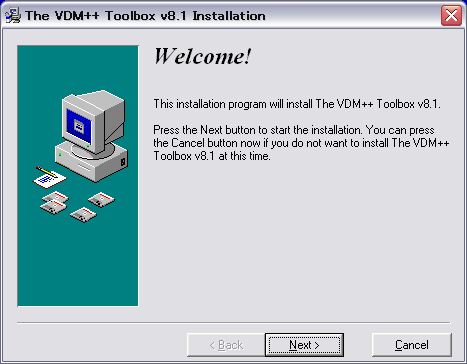
\includegraphics[scale=0.42, bb=0 0 467 364, clip]{install_pp_start.png}
\end{center}
#endif VDMPP
#ifdef VDMSL
\begin{center}
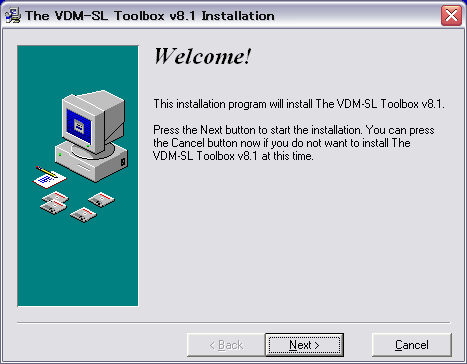
\includegraphics[scale=0.42, bb=0 0 467 364, clip]{install_sl_start.png}
\end{center}
#endif VDMSL
#ifdef VDMVICE
\begin{center}
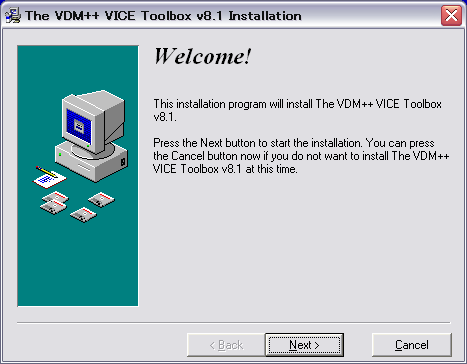
\includegraphics[scale=0.42, bb=0 0 467 364, clip]{install_vice_start.png}
\end{center}
#endif VDMVICE

\item 保存するディレクトリを選択し、『next』を押して次に進みます。
前に戻る場合は『back』を、インストールをキャンセルする場合は『Cancel』を押してください。

#ifdef VDMPP
\begin{center}
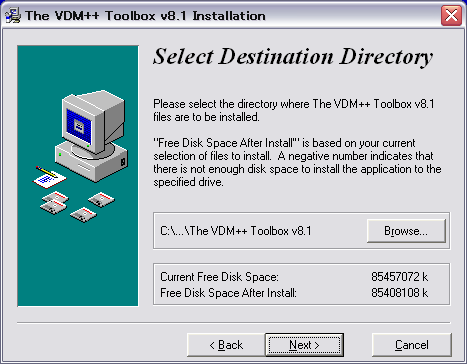
\includegraphics[scale=0.42,bb=0 0 467 364]{install_pp_second.png}
\end{center}
#endif VDMPP
#ifdef VDMSL
\begin{center}
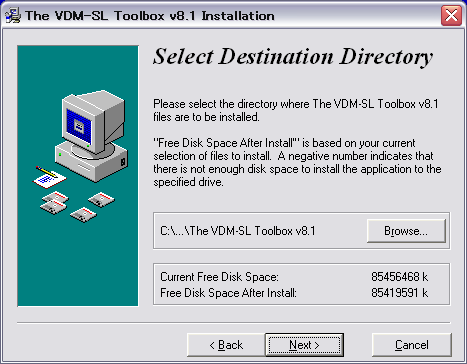
\includegraphics[scale=0.42,bb=0 0 467 364]{install_sl_second.png}
\end{center}
#endif VDMSL
#ifdef VDMVICE
\begin{center}
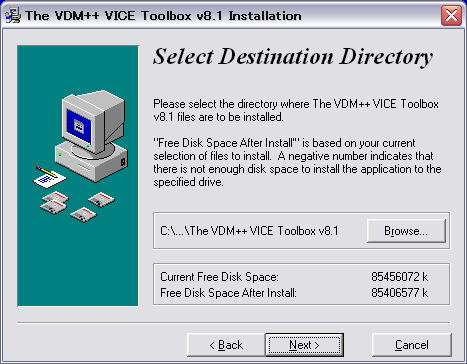
\includegraphics[scale=0.42,bb=0 0 467 364]{install_vice_second.png}
\end{center}
#endif VDMVICE

\item インストールを開始する場合は『next』を押して次に進みます。
前に戻る場合は『back』を、インストールをキャンセルする場合は『Cancel』を押してください。

#ifdef VDMPP
\begin{center}
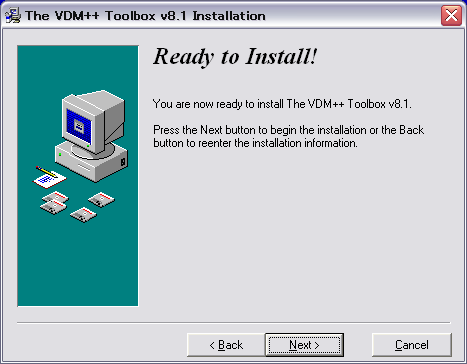
\includegraphics[scale=0.42,bb=0 0 467 364]{install_pp_third.png}
\end{center}
#endif VDMPP
#ifdef VDMSL
\begin{center}
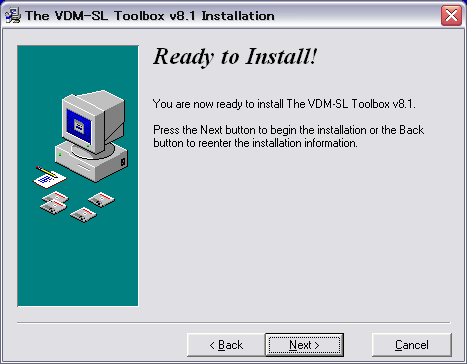
\includegraphics[scale=0.42, bb=0 0 467 364, clip]{install_sl_third.png}
\end{center}
#endif VDMSL
#ifdef VDMVICE
\begin{center}
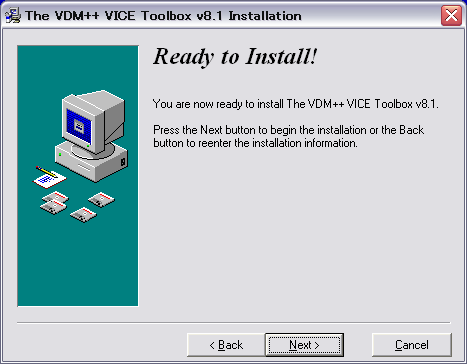
\includegraphics[scale=0.42, bb=0 0 467 364, clip]{install_vice_third.png}
\end{center}
#endif VDMVICE

\item 3.にて『next』を押すとインストールが始まり、進行状況が表示されます。

#ifdef VDMPP
\begin{center}
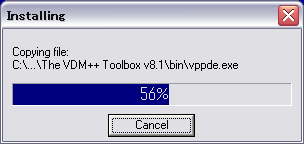
\includegraphics[scale=0.65,bb=0 0 304 144]{install_pp_bar.png}
\end{center}
#endif VDMPP
#ifdef VDMSL
\begin{center}
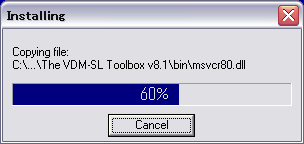
\includegraphics[scale=0.65,bb=0 0 304 144]{install_sl_bar.png}
\end{center}
#endif VDMSL
#ifdef VDMVICE
\begin{center}
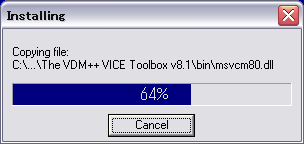
\includegraphics[scale=0.65,bb=0 0 304 144]{install_vice_bar.png}
\end{center}
#endif VDMVICE

\item インストールが終了したら、『Finish』を押してインストール完了です。

#ifdef VDMPP
\begin{center}
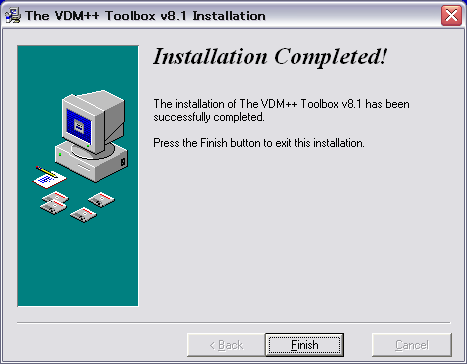
\includegraphics[scale=0.42,bb=0 0 467 364]{install_pp_finish.png}
\end{center}
#endif VDMPP
#ifdef VDMSL
\begin{center}
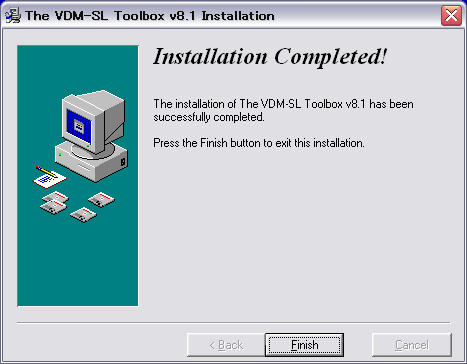
\includegraphics[scale=0.42,bb=0 0 467 364]{install_sl_finish.png}
\end{center}
#endif VDMSL
#ifdef VDMVICE
\begin{center}
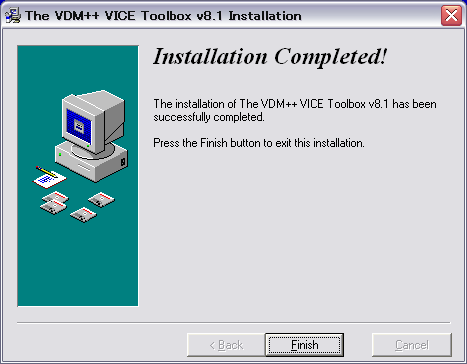
\includegraphics[scale=0.42,bb=0 0 467 364]{install_vice_finish.png}
\end{center}
#endif VDMVICE
\end{enumerate}

\subsection{VDMToolsの起動方法}
\Toolbox\ のインストール後、[スタート] - [全てのプログラム] 内に『\Toolbox\ 』が出来ます。
その中にインストールしたバージョンの\Toolbox\ がありますので、使用する\Toolbox\ を起動します。

#ifdef VDMPP
\subsection{Rational Rose : VDM++拡張のインストール}
すでにRational Rose(Rose 98 or Rose 2000)がWindows内にインストールされている場合、VDM++拡張は\Toolbox{}のインストール時に自動的に追加され、Rational RoseをWindowsレジストリに登録します。

Roseよりも先に\Toolbox{}のインストールを行った場合は、VDM++拡張をインストールするために以下の手順を行なう必要があります。

\begin{enumerate}
	\item Roseをインストールします。
	\item Roseのインストール後、【Program Files】 - 【The VDM++ Toolbox】 - 【{\tt uml}】フォルダ内に存在する
{\tt inst\_addin.exe}というファイル名のインストールプログラムを実行します。
{\tt inst\_addin.exe}実行時に、VDM++拡張はRational RoseをWindowsレジストリに登録します。
	\item Roseを再起動し、Roseの拡張管理メニューより拡張が作動するか確認してください。
\end{enumerate}
#endif VDMPP

#ifdef VDMVICE
\subsection{Rational Rose : VDM++拡張のインストール}
すでにRational Rose (Rose 98 or Rose 2000)がWindowsシステム内にインストールされているならば、VDM++拡張は \Toolbox{}をインストールしたときに自動的に追加されます。また、VDM++拡張はRational RoseをWindowsレジストリに登録します。

Roseよりも先に\Toolbox{}をインストールした場合は、VDM++拡張をインストールするために以下の手順を行なう必要があります。

\begin{enumerate}
	\item Roseをインストールします。
	\item Roseのインストール後、【Program Files】 - 【The VDM++ Toolbox】 - 【{\tt uml}】フォルダ内に存在する
{\tt inst\_addin.exe}というファイル名のインストールプログラムを実行します。
{\tt inst\_addin.exe}実行時に、VDM++拡張はRational RoseをWindowsレジストリに登録します。
	\item Roseを再起動し、Roseの拡張管理メニューより拡張が作動するか確認してください。
\end{enumerate}
#endif VDMVICE


\newpage
\section{Linuxプラットフォーム上でのインストール方法}
この章では、 \Toolbox\ をLinuxプラットフォーム上でインストールするための
手順を説明します。

\subsection{VDMToolsのインストールコピー}\label{purchinstall}
\begin{enumerate}
	\item \Toolbox を置くためにディレクトリを作成し、そこにバイナリファイルを置きます。(このマニュアルでは/home/ユーザ名/{\tt \vdmhome}を作成し、バイナリファイルを置きます。以下この仮定で進めます。)
	\item {\tt tar}コマンド等を用いてバイナリファイルを展開します。
	\item コマンドラインからVDMToolsを起動するためには、実行ファイルを標準のバイナリディレクトリに移動するか、 {\tt \vdmhome/bin} にパスを通します。以上で、準備は完了です。
\end{enumerate}

\subsection{VDMToolsの起動方法}
\subsubsection{CUIでの起動方法}
{\tt \vdmhome}/bin フォルダ内の{\tt \vdmde}を実行することで起動します。
\subsubsection{GUIでの起動方法}
{\tt \vdmhome}/bin フォルダ内の{\tt \vdmgde}を実行することで起動します。\\
※注意 libqt3-mtをインストールしていない場合には、事前にインストールしておきます。


\newpage
\section{Macプラットフォーム上でのインストール方法}
この章では、 \Toolbox\ をMacプラットフォーム上でインストールするための手順を説明します。

\subsection{VDMToolsのインストールコピー}\label{purchinstall}
\begin{enumerate}
	\item \Toolbox を置くためにディレクトリを作成し、そこにバイナリファイルを置きます。(このマニュアルでは/Application/{\tt \vdmtools}を作成し、バイナリファイルを置きます。以下この仮定で進めます。)
	\item {\tt tar}コマンド等を用いてバイナリファイルを展開します。
	\item コマンドラインからVDMToolsを起動するためには、実行ファイルを標準のバイナリディレクトリに移動するか、 {\tt \vdmtools/bin} にパスを通します。以上で、準備は完了です。
\end{enumerate}

\subsection{VDMToolsの起動方法}
\subsubsection{CUIでの起動方法}
/Applications/{\tt \vdmtools}/bin フォルダ内の{\tt \vdmde}を実行することで起動します。
\subsubsection{GUIでの起動方法}
/Applications/{\tt \vdmtools}//bin/{\tt \vdmgde}を実行することで起動します。
%※注意 libqt3-mtをインストールしていない場合には、事前にインストールしておきます。


\newpage
\section{Emacsインターフェースのインストール}
\label{sec:emacsinstall}

\begin{enumerate}
\item Emacsインターフェースのインストール
  
Emacsインターフェースを自身のサイト手順に従って、存在するEmacs環境に置くか、
ローカルディレクトリに移動することで、 {\tt emacs/\Index{\vdmdeNineteenEl}}
にEmacsインターフェースをインストールしてください。

\item  {\tt .emacs} ファイルのアップデート
  
{\tt \vdmdeNineteenEl} 内に読み込むために {\tt .emacs} ファイルをセットアップしてください。
もし、標準Emacs環境に {\tt emacs/\vdmdeNineteenEl} がある場合、 {\tt .emacs} へ以下の1行を加えなければなりません。

#ifdef VDMSL
\begin{verbatim}
  (autoload 'vdmde "vdmde" "" t)
\end{verbatim}
#endif VDMSL
#ifdef VDMPP
\begin{verbatim}
  (autoload 'vppde "vppde" "" t)
\end{verbatim}
#endif VDMPP
#ifdef VDMVICE
\begin{verbatim}
  (autoload 'vicede "vicede" "" t)
\end{verbatim}
#endif VDMVICE

その他に、 {\tt emacs/\vdmdeNineteenEl} へ以下のようにフルパスを加えなければなりません。

#ifdef VDMSL
\begin{verbatim}
  (autoload 'vdmde "/path/vdmde" "" t)
\end{verbatim}
#endif VDMSL
#ifdef VDMPP
\begin{verbatim}
  (autoload 'vppde "/path/vppde" "" t)
\end{verbatim}
#endif VDMPP
#ifdef VDMVICE
\begin{verbatim}
  (autoload 'vicede "/path/vicede" "" t)
\end{verbatim}
#endif VDMVICE
\end{enumerate}

\newpage
\section{新バージョンの取得方法}
\Toolbox\ の新バージョンがリリースされたときは、以下のVDM information \Index{Web site}
より取得することが出来ます。

\begin{verbatim}
#ifdef ENG
    http://www.vdmtools.jp/en
#endif ENG
#ifdef JPN
    http://www.vdmtools.jp/
#endif JPN
\end{verbatim}

\end{document}
